% ---------------------------------------------------------------------------
% Author guideline and sample document for EG publication using LaTeX2e input
% D.Fellner, v1.13, Jul 31, 2008

\documentclass{egpubl}
\usepackage{eg2015}

% --- for  Annual CONFERENCE
%\ConferenceSubmission   % uncomment for Conference submission
\ConferencePaper        % uncomment for (final) Conference Paper
% \STAR                   % uncomment for STAR contribution
% \Tutorial               % uncomment for Tutorial contribution
% \ShortPresentation      % uncomment for (final) Short Conference Presentation
% \Areas                  % uncomment for Areas contribution
% \MedicalPrize           % uncomment for Medical Prize contribution
% \Education              % uncomment for Education contribution
%
% --- for  CGF Journal
% \JournalSubmission    % uncomment for submission to Computer Graphics Forum
% \JournalPaper         % uncomment for final version of Journal Paper
%
% --- for  CGF Journal: special issue
% \SpecialIssueSubmission    % uncomment for submission to Computer Graphics Forum, special issue
% \SpecialIssuePaper         % uncomment for final version of Journal Paper, special issue
%
% --- for  EG Workshop Proceedings
% \WsSubmission    % uncomment for submission to EG Workshop
% \WsPaper         % uncomment for final version of EG Workshop contribution
%
 \electronicVersion % can be used both for the printed and electronic version

% !! *please* don't change anything above
% !! unless you REALLY know what you are doing
% ------------------------------------------------------------------------

% for including postscript figures
% mind: package option 'draft' will replace PS figure by a filname within a frame
%\ifpdf \usepackage[pdftex]{graphicx} \pdfcompresslevel=9
%\else \usepackage[dvips]{graphicx} \fi

\PrintedOrElectronic

% prepare for electronic version of your document
\usepackage{t1enc,dfadobe}

\usepackage{egweblnk}
\usepackage{cite}
\usepackage{balance}
\usepackage{multicol}

% For backwards compatibility to old LaTeX type font selection.
% Uncomment if your document adheres to LaTeX2e recommendations.
% \let\rm=\rmfamily    \let\sf=\sffamily    \let\tt=\ttfamily
% \let\it=\itshape     \let\sl=\slshape     \let\sc=\scshape
% \let\bf=\bfseries

% end of prologue

%\input{EGauthorGuidelines-body.inc}
% ---------------------------------------------------------------------
% EG author guidelines plus sample file for EG publication using LaTeX2e input
% D.Fellner, v1.17, Sep 23, 2010


\title[Exact GVD]%
      {Exact Generalized Voronoi Diagram computation using a sweepline algorithm}

% for anonymous conference submission please enter your SUBMISSION ID
% instead of the author's name (and leave the affiliation blank) !!
% For Computer Graphics Forum: Please use the abbreviation of your first name.

%% author example
%\author[D. Fellner \& S. Behnke]
%       {D.\,W. Fellner\thanks{Chairman Eurographics Publications Board}$^{1,2}$
%        and S. Behnke$^{2}$
%        S. Spencer$^2$\thanks{Chairman Siggraph Publications Board} \\
%         $^1$TU Darmstadt \& Fraunhofer IGD, Germany \\
%         $^2$Institut f{\"u}r ComputerGraphik \& Wissensvisualisierung, TU Graz, Austria
%       }

\author[J. Edwards \& Daniel Marsden]
%       {John Edwards\thanks{jedwards@sci.utah.edu}$^1$ and
       {John Edwards$^1$ and
         Daniel Marsden$^1$ \\
         \parbox[t]{10cm}{\centering $^1$Utah State University}
       }
%\author[paper1040]
%       {paper1040}

% ------------------------------------------------------------------------

% if the Editors-in-Chief have given you the data, you may uncomment
% the following five lines and insert it here
%
% \volume{27}   % the volume in which the issue will be published;
% \issue{1}     % the issue number of the publication
% \pStartPage{1}      % set starting page

\renewcommand{\paragraph}[1]{\noindent \textbf{#1}}
%\usepackage{amsmath,amsthm,amsfonts,amscd,amssymb,amstext} 
\usepackage{amsmath,amsfonts,amscd,amssymb,amstext} 
\usepackage{mathrsfs}
				% Some packages to write mathematics.
\usepackage{overpic}
\usepackage{eucal} 	 	% Euler fonts
\usepackage{verbatim}      	% Allows quoting source with commands.
\usepackage{makeidx}       	% Package to make an index.
%\usepackage{citesort}         	% 
\usepackage{subfig}
\usepackage{graphicx}
\usepackage{url}		% Allows good typesetting of web URLs.
\usepackage{multirow}
%\usepackage[linesnumbered, noline]{algorithm2e}
%\usepackage[boxed, noline]{algorithm2e}
\usepackage[ruled]{algorithm2e}
\usepackage{booktabs}
\usepackage{tabularx}
\usepackage{array}
\usepackage{color}
\usepackage{tikz}
% To balance the columns at the end
\usepackage{balance}
\usepackage[mediumspace,mediumqspace,Grey,squaren]{SIunits}
%\usepackage{draftcopy}		% Uncomment this line to have the
				% word, "DRAFT," as a background
				% "watermark" on all of the pages of
				% of your draft versions. When ready
				% to generate your final copy, re-comment
				% it out with a percent sign to remove
				% the word draft before you re-run
				% Makediss for the last time.
\usepackage[normalem]{ulem}

\definecolor{bostonuniversityred}{rgb}{0.8, 0.0, 0.0}

%------------------------------------------------------------
% Custom commands
%------------------------------------------------------------
%\newcommand{\old}[1]{\textcolor{blue}{\sout{#1}}}
\newcommand{\old}[1]{}

%\newcommand{\red}[1]{\textcolor{red}{#1}}
%\newcommand{\red}[1]{\textcolor{bostonuniversityred}{#1}}
\newcommand{\red}[1]{#1}

%\newcommand{\reconstruct}{RECONSTRUCT\textsuperscript{\texttrademark}}
%\newcommand{\tm}{\textsuperscript{\texttrademark}}
\newcommand{\tm}{$^1$}
\newcommand{\addref}{\red{REF}}
\newcommand{\mathtext}[1]{\text{#1}}
\newcommand{\etal}{et al.\ }
\newcommand{\algorithmspace}{\vspace{8pt}}
\newcommand{\glfs}{\emph{glfs}}

\renewcommand{\vec}[1]{\mathbf{#1}}

\newcommand{\centercell}[1]{\multicolumn{1}{c}{#1}}
\newcolumntype{x}[1]{>{\centering\arraybackslash\hspace{0pt}}m{#1}}
\newcolumntype{y}[1]{>{\centering\arraybackslash\hspace{0pt}}m{#1\textwidth}}
\newcolumntype{M}{>{\centering\arraybackslash}m{1cm}}

\DeclareMathOperator*{\argmin}{arg\,min}
\DeclareMathOperator*{\argmax}{arg\,max}

\newcommand{\BigO}[1]{\ensuremath{\operatorname{O}\left(#1\right)}}
\newcommand{\centroid}{\mathscr{C}}
\newcommand{\iring}{\mathscr{R}}

% aligned
\renewcommand{\d}{\delta}
\newcommand{\vempty}{\mathscr{E}}
\newcommand{\e}{\epsilon}
\newcommand{\dist}{\mathtext{dist}}
\newcommand{\ball}{\mathscr{B}}


\newcommand{\hgt}{22mm}

%--------------------------------------------------
% Theorem environments (amsthm package required)
%--------------------------------------------------
% \theoremstyle{plain} %% This is the default
\newtheorem{theorem}{Theorem}
\newtheorem{lemma}{Lemma}
\newtheorem{corollary}{Corollary}
\newtheorem{conjecture}{Conjecture}
\newtheorem{crit}{Criterion}
\newtheorem{condition}{Condition}
\newtheorem{fact}{Fact}

%\theoremstyle{definition}
%\newtheorem{defn}{Definition}[section]

%\theoremstyle{remark}
%\newtheorem{rem}{Remark}[section]
%\newtheorem*{notation}{Notation}

%\numberwithin{equation}{section}

%--------------------------------------------------
% Tight enumerations
%--------------------------------------------------
\newenvironment{tightenumerate}{
\begin{enumerate}
  \setlength{\itemsep}{1pt}
  \setlength{\parskip}{0pt}
  \setlength{\parsep}{0pt}
}{\end{enumerate}
}
\newenvironment{tightitemize}{
\begin{itemize}
  \setlength{\itemsep}{1pt}
  \setlength{\parskip}{0pt}
  \setlength{\parsep}{0pt}
}{\end{itemize}
}

%--------------------------------------------------
% Add figs to graphics path
%--------------------------------------------------
\graphicspath{{./}{./figs/}}

\newcolumntype{H}{@{}>{\lrbox0}l<{\endlrbox}}


%-------------------------------------------------------------------------
\begin{document}
%\begin{multicols}{3}
%\end{multicols}
	
%\teaser{
%  \subfloat[][]{
%    \label{fig:gears1}
%    \begin{tikzpicture}
%      \node[anchor=south west,inner sep=0] at (0,0) {
%        \begin{tabular}[b]{c}
%          \includegraphics[height=0.8in]{gears-far1.png} \\
%          \includegraphics[height=0.8in]{gears-close1.png}
%        \end{tabular}
%      };
%      \draw[black,thick] (1.4,3.2) rectangle (2.0,3.6);
%      \draw[black,dashed] (1.4,3.6) -- (0.22,2.15);
%      \draw[black,dashed] (2.0,3.6) -- (2.95,2.15);
%      \draw[black,thick] (0.22,0.1) rectangle (2.95,2.15);
%    \end{tikzpicture}
%  }
%  \subfloat[][]{
%    \label{fig:gears}
%    \begin{tikzpicture}
%      \node[anchor=south west,inner sep=0] at (0,0) {
%        \begin{tabular}[b]{c}
%          \includegraphics[height=0.8in]{gears-far4.png} \\
%          \includegraphics[height=0.8in]{gears-close4.png}
%        \end{tabular}
%      };
%      \draw[black,thick] (1.3,3.1) rectangle (1.9,3.5);
%      \draw[black,dashed] (1.3,3.5) -- (0.22,2.15);
%      \draw[black,dashed] (1.9,3.5) -- (2.92,2.15);
%      \draw[black,thick] (0.22,0.1) rectangle (2.92,2.15);
%    \end{tikzpicture}
%  }
%  \hspace{3mm}
%  \subfloat[][]{
%    \label{fig:knife}
%    \includegraphics[trim=4cm 0cm 4cm 2.5cm, clip=true, height=1.4in]
%                    {knife-above/slice-00000.png}
%  }
%  \subfloat[][]{
%    \label{fig:knife2}
%    \includegraphics[trim=2mm 0cm 2mm 2cm, clip=true, height=1.4in]
%                    {knife-above/slice-00110.png}
%  }
%  \caption{Two example applications of the \red{approximated} generalized Voronoi diagram (GVD) computed by our novel, adaptive algorithm. Previous GVD methods require a gridded space of $2^{24}$ (gears dataset) and $2^{36}$ (knives dataset) voxels to resolve the closely spaced objects.
%    \protect\subref{fig:gears1} Two gears with regions of very tight spacing.
%    \protect\subref{fig:gears} The GVD of the gears model.  The surface is colored red in areas of very close tolerance.
%    \protect\subref{fig:knife} Three butter knives in a wood block.  To animate removal of the knives without intersecting the block requires extreme care because of close mesh spacing.
%    \protect\subref{fig:knife2} Intersection-free motion is guaranteed by computing motion vectors based on the GVD and allowing motion only within a Voronoi cell.
%  }
%  \label{fig:teaser}
%}

\maketitle

\begin{abstract}
We introduce a geometric algorithm that allows the Generalized Voronoi Diagram to be created using a sweepline. In this generalized version the algorithm accepts input that includes any non-overlapping simple polygons including lines and points. From the input, the algorithm uses the sweepline approach to produce the Voronoi Diagram with $O(n logn)$ worst-case run-time. 

%   Leave one blank line after the abstract, 
%   then add the subject categories according to the ACM Classification Index 
%   (see http://www.acm.org/class/1998/).

\begin{classification} % according to http://www.acm.org/class/1998/
% any clasification items here
\end{classification}

\end{abstract}

%-------------------------------------------------------------------------
% Body
%-------------------------------------------------------------------------

%-------------------------------------------------------------------------------
% introduction
%-------------------------------------------------------------------------------
\section{Introduction}
\label{sec:intro}

Place introduction here

%\paragraph{Main contributions} In computation of a GVD, we are less concerned with details of objects; rather, we adapt subdivision to most efficiently compute a distance field for GVD computation.  Our main contributions are fourfold.\footnote{Our algorithms support both 2D and 3D. For simplicity, we will use 3D terms (e.g. octree rather than quadtree) when discussing dimension-independent concepts, but will revert to 2D terms when convenient.}

\paragraph{Main contributions} Place Contributions Here 
% Example The three primary technical contributions described in the paper are as follows.

\begin{enumerate}
\item Items here
\end{enumerate}


%-------------------------------------------------------------------------------
% Related work
%-------------------------------------------------------------------------------
\section{Related work}
Place related work here


%\paragraph{Generalized Voronoi diagrams}
%A theoretical framework for generalized Voronoi diagrams can be found in Boissonnat \etal \shortcite{boissonnat2006curved}. Ordinary Voronoi diagrams are well studied and efficient algorithms exist that compute them exactly \cite{de2008computational}, but exact algorithms for the generalized Voronoi diagram are limited to a small set of special cases \cite{lee1982medial,karavelas2004robust}. In an early work, Lavender \etal \shortcite{lavender1992voronoi} define and compute GVDs over a set of solid models using an octree.  Etzion and Rappoport \shortcite{etzion2002computing} represent the GVD bisector symbolically for lazy evaluation, but are limited to sites that are polyhedra.  Boada \etal \shortcite{boada2002voronoi,boada2008approximations} use an adaptive approach to GVD computation, but their algorithm is restricted to GVDs with connected regions and is inefficient for polyhedral objects with many facets.  Two other works are adaptive \cite{teichmann1997polygonal,vleugels1998approximating} but are computationally expensive and are restricted to convex sites.

%-----------------------------------------------------------
% Sweepline Algorithm
%-----------------------------------------------------------
\section{Sweepline Algorithm}
\label{sec:sweepline-algorithm}

 Place algorithm section here

\algorithmspace
\begin{algorithm}
  \DontPrintSemicolon
%  \LinesNumbered
  \KwIn{events}
  \BlankLine
  \tcp{Initialization}
  $beachline$ := the set of arc nodes\;
  $closeEventPoints$ := the set of all close events\;
  $events$ := a priority queue of sorted points or sites\;
  \While{$events$ > 0}{
  	let $e$ := next event in $events$ by popping of the top\;
  	move the sweepline to include point $e$\;
    
    \If{$e$ is a close event}{
    	\If{$e$ is live}{
    	  update the associated arc node to close on point $e$\;
    	  remove the arc node from the $beachline$ and return $newEvents$\;
    	  
    	  \ForEach{$ev$ in $newEvents$}{
    	  	\If {$ev$ is below $e$}{
    	  		add $ev$ to $events$ in sorted order\;
    	  		\If{$ev$ is a close event}{
    	  			add $ev$ to $closeEventPoints$
    	  		}
    	  	}
    	  }
    	  
		}
   	}
    \Else{
   	  \tcp{Site event}
   	  add $e$ to the $beachline$ and return $newEvents$
   	   \ForEach{$ev$ in $newEvents$}{
   	  	\If {$ev$ is below $e$}{
   	  		add $ev$ to $events$ in sorted order\;
   	  		\If{$ev$ is a close event}{
   	  			add $ev$ to $closeEventPoints$
   	  		}
   	  	}
   	  }
    }
  }
\caption{Sweepline Algorithm}
\label{alg:sweepline-algorithm}
\end{algorithm}
\algorithmspace

\begin{figure}
  \centering
  \subfloat[][]{
    \label{fig:sweepA}
    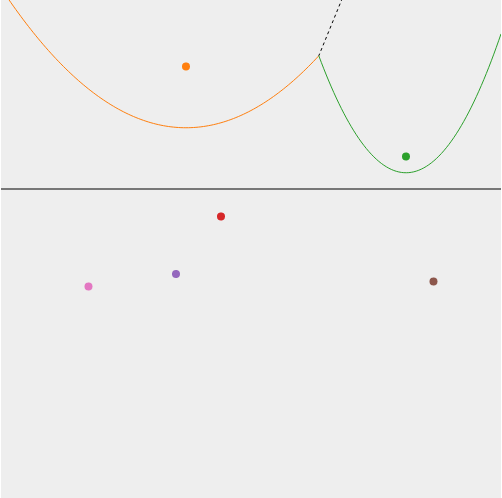
\includegraphics[width=0.32\columnwidth]{fig1_a.png} }
  \subfloat[][]{
    \label{fig:sweepB}
    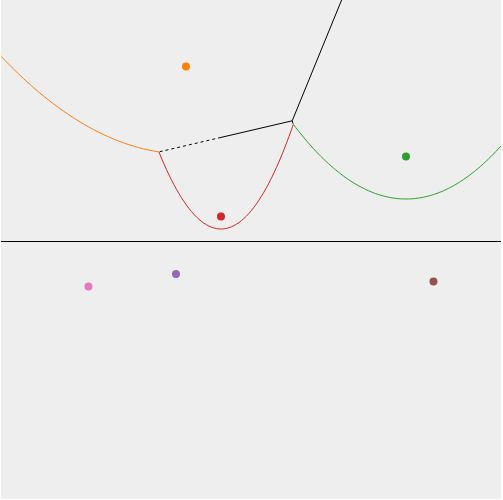
\includegraphics[width=0.32\columnwidth]{fig1_b.png} }
  \subfloat[][]{
    \label{fig:sweepC}
    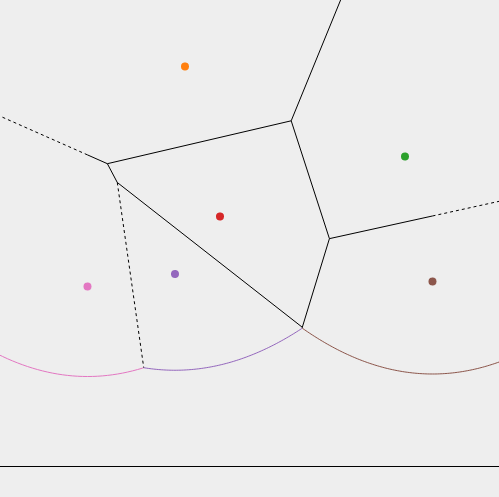
\includegraphics[width=0.32\columnwidth]{fig1_c.png} } \\
  \subfloat[][]{
    \label{fig:sweepD}
    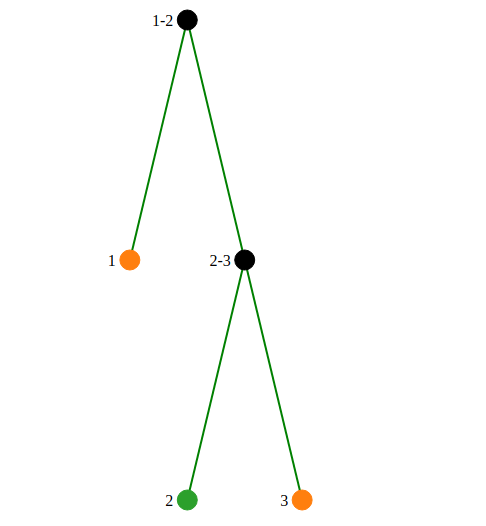
\includegraphics[width=0.32\columnwidth]{fig1_d.png} }
  \subfloat[][]{
    \label{fig:sweepE}
    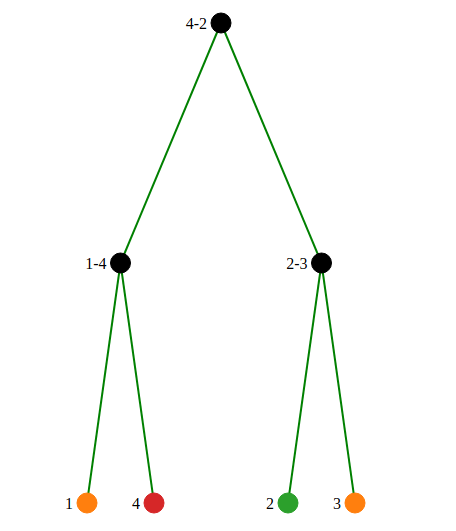
\includegraphics[width=0.32\columnwidth]{fig1_e.png} }
  \subfloat[][]{
    \label{fig:sweepF}
    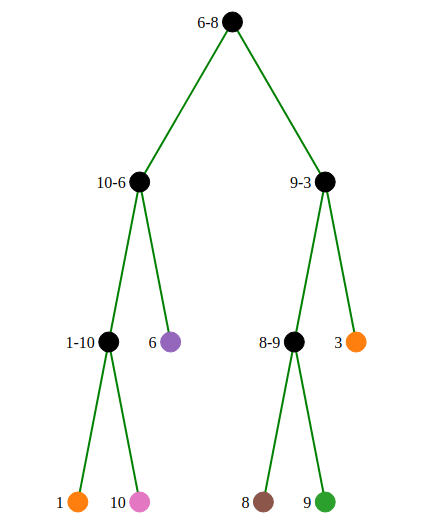
\includegraphics[width=0.32\columnwidth]{fig1_f.png} }
  \caption{Sweepline Algorithm
    \protect\subref{fig:sweepA} Here the algorithm has processed the first two events and multiple arc nodes have been added to the beach line, in which the leaf nodes represent active sites and the parent nodes are edge connections (as shown in \protect\subref{fig:sweepD}). It is important to note the beach line includes the edge connection 2-3 even though it is not shown here. The line created by this connection is the same as that made by 1-2.
    \protect\subref{fig:sweepB} Once the algorithm is able to triangulate a close event, it removes the arc node that formed it. This is illustrated in \protect\subref{fig:sweepE} where there is no longer an edge connection between 1-2 or 4-1.
    \protect\subref{fig:sweepC} When a site is enclosed completely by vertexes it is removed entirely from the beach line (as shown in \protect\subref{fig:sweepF}).
  }
  \label{fig:sweepline}
\end{figure}


\begin{figure}
	\centering
	\subfloat[][]{
		\label{fig:live_event}
		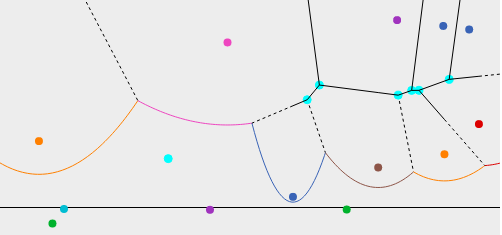
\includegraphics[width=0.52\columnwidth]{fig2_a.png} }
	\subfloat[][]{
		\label{fig:live_event_tree}
		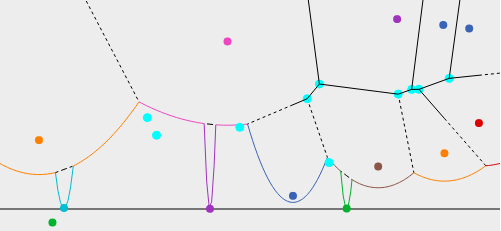
\includegraphics[width=0.52\columnwidth]{fig2_b.png} } \\
	\subfloat[][]{
		\label{fig:non_live}
		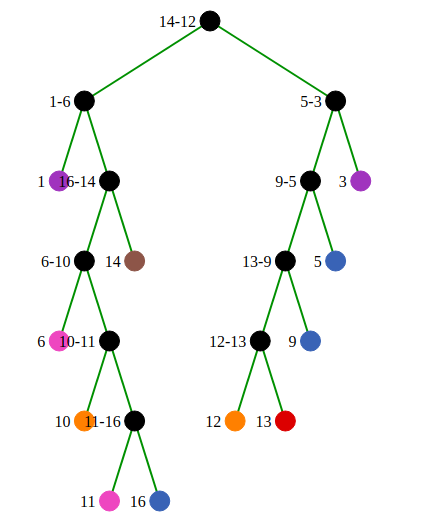
\includegraphics[width=0.52\columnwidth]{fig2_c.png} }
	\subfloat[][]{
		\label{fig:non_live_tree}
		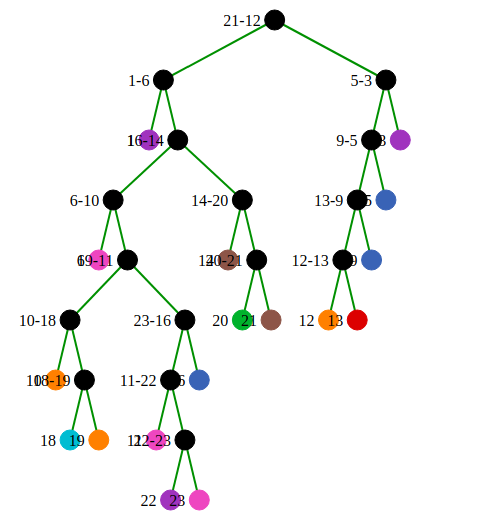
\includegraphics[width=0.52\columnwidth]{fig2_d.png} }
	\caption{Illustration of live and non-live close events 
		\protect\subref{fig:live_event} Here lets examine nodes 16 and 11. It is known that a close event will occur where nodes 16, 11, and 10 arcs' will meet. Let's name this close event A.
		\protect\subref{fig:live_event_tree} Before we completely come to close on event A, node 22 gets added to the beach line and generates two new events. This causes  close event A to split into two new close events and therefore is considered a non-live close event. 
	}
	\label{fig:live_events}
\end{figure}

\begin{figure}
	\centering
	\subfloat[][]{
		\label{fig:close_eventA}
		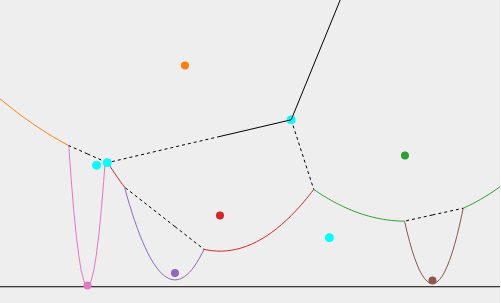
\includegraphics[width=0.52\columnwidth]{fig3_a.png} }
	\subfloat[][]{
		\label{fig:close_eventB}
		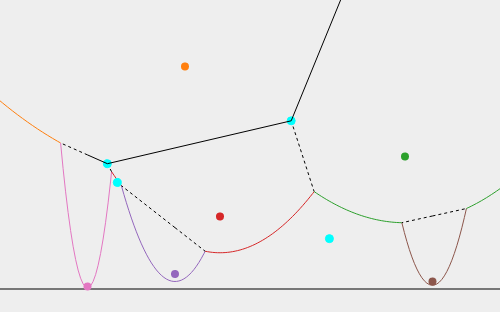
\includegraphics[width=0.52\columnwidth]{fig3_b.png} } \\
	\subfloat[][]{
		\label{fig:close_eventC}
		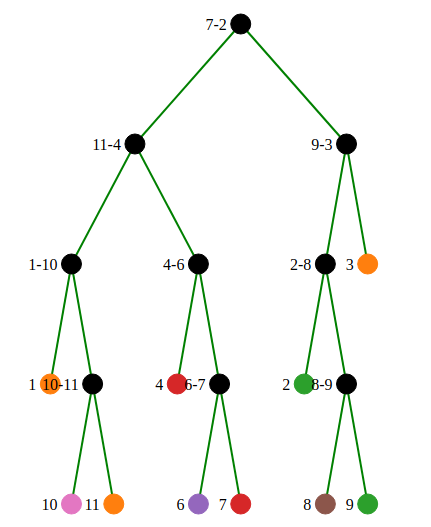
\includegraphics[width=0.52\columnwidth]{fig3_c.png} }
	\subfloat[][]{
		\label{fig:close_eventD}
		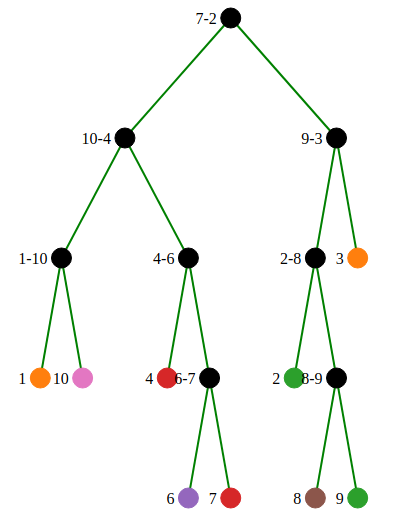
\includegraphics[width=0.52\columnwidth]{fig3_d.png} }
	\caption{Illustration of close event generated from a close event
		\protect\subref{fig:close_eventA} Lets note the close event generated from node 10 closing with nodes 11 and 4. Lets name this close event B.
		\protect\subref{fig:close_eventB} Once event B is defined node 10 no longer creates an arc with node 11 and is removed. In this removal node 10's arc now maps to node 4's arc instead. As this happens a new close event is generated by arcs from nodes 11, 4 and 6.
	}
	\label{fig:close_events}
\end{figure}

%-------------------------------------------------------------------------------
% Generalized Sites
%-------------------------------------------------------------------------------

\begin{figure}
	\centering
	\subfloat[][]{
		\label{fig:gvd1}
		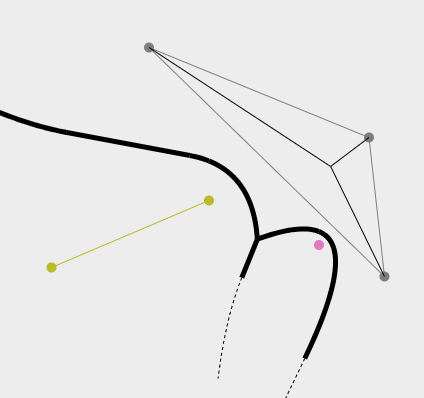
\includegraphics[width=0.5\columnwidth]{gvd_1.png} }
	\caption{Generalized Sites
		\protect\subref{fig:gvd1} The exact Generalized Voronoi Diagram(GVD) is produced as sweep-line processes generalized sites. The algorithm supports any number of simple polygons as long as they are not overlapping. Each polygon is made up of a number of connected points. The GVD algorithm computes the appropriate bisector between sites. The bisector represents the continuous parabola or line that separates sites. If a point lies at the end of a segment the bisector is a line perpendicular to the segment intersecting that point; otherwise, the bisector between a point site and a segment site is a parabola representing the bisector of the two sites. With a pair of segments their bisector can include up to 2 lines if the intersection of the two segments lies between the endpoints of one segment. In all other cases the bisector of two segments can be represented with a single line.
	}
	\label{fig:gvd}
\end{figure}


\begin{figure}
	\centering
	\subfloat[][]{
		\label{fig:gvd2}
		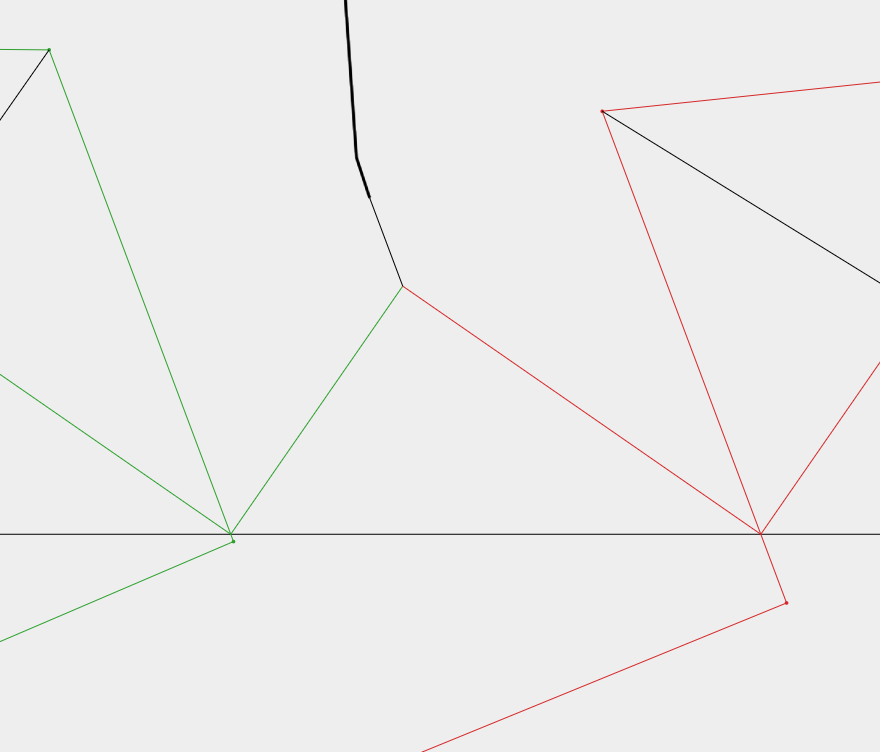
\includegraphics[width=0.5\columnwidth]{gvd_2.png} }
	\caption{Special Cases
		\protect\subref{fig:gvd2} Special cases such as parallel sites are handled as the algorithm computes the correct bisector between each site. Between a pair of segments we use their intersection to find the bisector, however, when the segments are parallel there is no intersection and we use the average of the segments to determine the bisector. Finding the correct bisector enables the algorithm to determine future close events. 
	}
	\label{fig:gvd}
\end{figure}

%-------------------------------------------------------------------------------
% Results
%-------------------------------------------------------------------------------

%-------------------------------------------------------------------------------
% Conclusions
%-------------------------------------------------------------------------------
\section{Conclusions}

%-------------------------------------------------------------------------------
% Acknowledgements
%-------------------------------------------------------------------------------
\section*{Acknowledgments}
%Thanks to Kristen Harris for use of the neuronal data and Jonathan Bronson for the heart data. The work of JE and VP was supported in part by NSF IIS-1314896, NSF ACI-0904631, DOE/NEUP 120341, DOE/UV-CDAT DESC0006872, DOE/Codesign P01180734, DOE/SciDAC DESC0007446, DOE/PIPER DESC0010498, and DOE/CCMSC DENA0002375. This work initiated at the University of Texas when JE, ED  and CB were supported in part by NIH contract R01-EB00487, NSF Grant OCI-1216701 and SNL contract 1439100.

%-------------------------------------------------------------------------
% Bibliography
%-------------------------------------------------------------------------

%\bibliographystyle{eg-alpha}
%\bibliographystyle{eg-alpha-doi}
%\balance
%\bibliography{paper}

\end{document}
